\chapter{REFERENCIAL TEÓRICO}

\section{GESTÃO DE DOCUMENTOS MÉDICOS}

A digitalização de documentos médicos possui um papel fundamental na modernização dos processos da área da saúde, tornando-se essencial na melhoria da organização, segurança e acessibilidade de informações de pacientes \cite{pereira2024toward}. Conforme aponta \citeonline{hage2023plataforma}, a troca dos tradicionais registros em papel para registros digitais traz facilidades no compartilhamento de informações entre diferentes instituições e profissionais, como hospitais, clínicas, centros de pesquisa e consultórios particulares.

O processo de digitalização de documentos assume um papel fundamental na área da psicologia, pois a privacidade das informações dos pacientes é de extrema importância tendo em vista que seus maiores segredos e traumas são expostos nas seções, os quais são transcritos nos chamados “relatos de seção” \cite{salles2023privacidade}.

Ao armazenarmos os documentos de forma eletrônica acabamos ganhando um maior controle de acesso a estes registros, garantindo que apenas quem possui as devidas autorizações possam visualizar e modificar as informações. Além disso, temos uma maior organização dos documentos, o que por sua vez acaba contribuindo para uma maior eficiência no fluxo de trabalho dos profissionais \cite{moerschberger2017reflexoes}.

Em sua tese \citeonline{hage2023plataforma} fala que a troca dos clássicos registros em papel por registros eletrônicos minimiza problemas relacionados à gestão de documentos, como por exemplo arquivos duplicados, erros de preenchimento e a dificuldade e demora para recuperar esses documentos. Há relatos de que antes da adoção de sistemas digitais em clínicas e hospitais, o preenchimento manual de documentos importantes frequentemente resultava em erros no preenchimento de falhas na organização e em alguns casos até mesmo na perda dos registros. Esses problemas relacionados à gestão de documentos acaba sendo ainda mais evidente na psicologia clínica, onde todas as seções geram documentos, e o acesso a esses registros pelos profissionais é de suma importância para o acompanhamento histórico dos pacientes e da evolução clínica dos mesmos ao longo de cada sessão \cite{opsi2025}.

Além da digitalização dos documentos trazer o benefício de uma organização mais otimizada, eleva a segurança destes documentos ao prevenir acessos não autorizados e reduz o risco de perda de documentos devido a extravios ou até mesmo a própria deterioração física dos arquivos. \citeonline{hage2023plataforma} também acrescenta que a centralização dos dados em uma plataforma pode contribuir para uma análise mais aprimorada das informações contidas nos documentos e com isso possibilitar que psicólogos, ou outros profissionais, possam identificar padrões ao fazer a análise do histórico dos seus pacientes.

Como mencionado, um ponto essencial da gestão de documentos médicos é a proteção das informações dos pacientes. Em sua tese \citeonline{hage2023plataforma} enfatiza a necessidade de implementar mecanismos de criptografia para assegurar a integridade dos dados salvos em plataformas digitais, o autor afirma que esta estratégia pode prevenir acessos não autorizados e reduzir a possibilidade de ataques cibernéticos. Especificamente falando de registros psicológicos, essa proteção se torna ainda mais crítica, uma vez que tais documentos frequentemente contêm relatos pessoais e informações detalhadas sobre a saúde mental dos pacientes, exigindo medidas rigorosas de segurança e confidencialidade.

\section{CRIPTOGRAFIA E SEGURANÇA DA INFORMAÇÃO}

A segurança da informação é um assunto de extrema importância na atualidade onde temos um crescente aumento da digitalização de documentos importantes,͏ como os documentos médicos por exemplo, onde a confidencialidade destes arquivos é essencial para preservar as informações pessoais dos pacientes. 

\citeonline{viana2022criptografia} destaca que devido a crescente dependência da sociedade por tecnologia e consequentemente o aumento do tráfego de informações nas redes se faz necessário soluções robustas para a proteção dos dados sensíveis que estão disponíveis na rede, dados como prontuários médicos ou relatos de uma seção psicológica. Uma ferramenta essencial para essa proteção é a criptografia, ela pode garantir a integridade, autenticidade e confidencialidade dessas informações disponíveis na rede.

\subsection{Princípios da Segurança da Informação}

A segurança da informação está fundamentada em três princípios fundamentais, que em seu artigo \citeonline{viana2022criptografia} apresenta como a tríade CIA: confidencialidade, integridade e disponibilidade.

O princípio da confidencialidade assegura que os dados estarão acessíveis somente para os usuários que possuírem as devidas autorizações. Segundo \citeonline{viana2022criptografia}, a criptografia desempenha um papel crucial nesse princípio ao transformar as informações  salvas em um formato ilegível para qualquer pessoa que não possua a chave de descriptografia. Isso é essencial para proteger registros médicos de acessos não autorizados.

Integridade é a garantia que os dados não serão alterados indevidamente durante o armazenamento ou a transmissão. No contexto da plataforma proposta neste trabalho, a integridade impede modificações não autorizadas em relatórios psicológicos e laudos médicos. Segundo \citeonline{viana2022criptografia}, os algoritmos criptográficos modernos são projetados para detectar qualquer alteração indevida nas informações protegidas.

Por fim temos a disponibilidade, que está mais associada à manutenção de uma infraestrutura robusta e confiável que seja capaz de assegurar que os dados estejam sempre acessíveis para usuários autorizados sempre que necessário.\citeonline{viana2022criptografia} destacam que a  criptografia não está diretamente ligada à disponibilidade, entretanto, a disponibilidade de dados para as pessoas autorizadas é um dos princípios da segurança da informação e por isso é de extrema importância ter isso em mente ao planejar qualquer sistema. No caso da plataforma proposta neste trabalho, garantir a disponibilidade significa permitir que psicólogos acessem prontuários e documentos médicos sempre que necessário, sem comprometer a segurança dos dados.

Além da tríade CIA citada anteriormente, \citeonline{viana2022criptografia} incluiu em seu artigo a legalidade, auditabilidade e não repúdio de autoria.

A legalidade na segurança da informação diz respeito à adequação das políticas de proteção de dados às legislações e regulamentações em vigor, garantindo conformidade com contratos e normas estabelecidas. Já a auditabilidade e o não repúdio estão relacionados à integridade e rastreabilidade das informações. A auditabilidade refere-se ao registro detalhado de acessos e operações realizadas, permitindo a identificação dos responsáveis por modificações nos dados. O não repúdio, por sua vez, assegura que um usuário não possa negar a autoria de uma ação ou alteração, por meio de mecanismos que comprovam a autenticidade das interações realizadas

\subsection{Criptografia Simétrica}

A criptografia simétrica caracteriza-se pelo uso de uma única chave tanto para a cifragem quanto para a decifragem dos dados. Dessa forma, emissor e receptor devem compartilhar previamente essa chave secreta para assegurar a confidencialidade da comunicação. Conforme destacado por \citeonline{viana2022criptografia}, essa abordagem apresenta vantagens em termos de eficiência e velocidade, porém enfrenta desafios relacionados à necessidade de um meio seguro para o compartilhamento da chave.

Os principais algoritmos de criptografia simétrica mencionados no estudo incluem:

\begin{itemize}
    \item DES (Data Encryption Standard) – Desenvolvido em 1977, foi amplamente utilizado, mas atualmente é considerado vulnerável devido ao tamanho reduzido de sua chave (56 bits), o que o torna suscetível a ataques de força bruta \cite{viana2022criptografia}.
    \item 3DES (Triple DES) – Variante do DES que aplica o processo de criptografia três vezes consecutivas, aumentando a segurança, porém com um impacto negativo no desempenho em comparação a algoritmos mais modernos \cite{viana2022criptografia}.
    \item AES (Advanced Encryption Standard) – Um dos algoritmos mais adotados globalmente, utilizado por instituições governamentais e corporativas. Opera com chaves de 128, 192 ou 256 bits, garantindo alto nível de segurança e desempenho. Segundo \citeonline{viana2022criptografia}, o AES é reconhecido como um dos métodos mais confiáveis na atualidade.
    \item Blowfish – Algoritmo de chave simétrica que processa blocos de 64 bits e permite chaves de 32 a 448 bits. Destaca-se por sua eficiência e segurança, sendo empregado em diversas aplicações, especialmente no armazenamento seguro de dados \cite{viana2022criptografia}.
    \item Twofish – Evolução do Blowfish, suporta chaves de até 256 bits e é utilizado em sistemas que demandam criptografia robusta e eficiente \cite{viana2022criptografia}.
\end{itemize}

Embora a criptografia simétrica seja vantajosa em cenários que exigem rapidez no processamento, a necessidade de compartilhamento seguro da chave representa um ponto vulnerável. Ataques como a interceptação da chave podem comprometer a segurança do sistema, exigindo a adoção de mecanismos adicionais de proteção \cite{viana2022criptografia}.

\subsection{Criptografia Assimétrica}

A criptografia assimétrica distingue-se da simétrica por empregar um par de chaves distintas: uma chave pública, utilizada para cifrar os dados, e uma chave privada, necessária para decifrá-los. Esse modelo elimina a exigência de compartilhar uma chave secreta única, o que aprimora a segurança das comunicações \cite{viana2022criptografia}.

Entre os principais algoritmos de criptografia assimétrica abordados no estudo, destacam-se:

\begin{itemize}
    \item RSA (Rivest-Shamir-Adleman) – Considerado um dos algoritmos mais amplamente adotados, sua segurança baseia-se na dificuldade de fatoração de números primos extremamente grandes. Esse fator torna a decodificação impraticável sem a posse da chave privada. Segundo \citeonline{viana2022criptografia}, o RSA é amplamente empregado na segurança digital, em assinaturas eletrônicas e na proteção de informações sigilosas.
    \item Diffie-Hellman – Embora não seja propriamente um algoritmo de criptografia, trata-se de um protocolo voltado à troca segura de chaves entre partes comunicantes em ambientes não confiáveis \cite{viana2022criptografia}.
    \item ElGamal – Baseado na complexidade do problema do logaritmo discreto, esse algoritmo proporciona um elevado nível de segurança e é frequentemente utilizado na geração de assinaturas digitais e na proteção de dados criptografados \cite{viana2022criptografia}.
\end{itemize}

Apesar das vantagens em termos de segurança, a criptografia assimétrica apresenta um desempenho inferior ao da criptografia simétrica, devido ao alto custo computacional de suas operações matemáticas. Para contornar essa limitação, muitas aplicações adotam um modelo híbrido, no qual o algoritmo AES (simétrico) é empregado para criptografar os dados, enquanto o RSA (assimétrico) é utilizado na troca segura das chaves \cite{viana2022criptografia}.

\section{ASSINATURA DIGITAL}
\subsection{Conceitos Fundamentais}

A assinatura digital é um mecanismo criptográfico que assegura a integridade, a autenticidade e o não repúdio de documentos eletrônicos. Ela funciona com base em algoritmos de chave pública e privada, sendo esta última utilizada para assinar o documento, enquanto a chave pública é empregada para verificar sua autenticidade \cite{brasil2001medida}. A principal tecnologia por trás da assinatura digital é a Infraestrutura de Chaves Públicas Brasileira (ICP-Brasil), que oferece a base legal e técnica para a emissão e verificação de certificados digitais no país.

Segundo o Instituto Nacional de Tecnologia da Informação (ITI), a assinatura digital “é o resultado da aplicação de um processo matemático (algoritmo) a um documento eletrônico utilizando uma chave criptográfica privada associada a um certificado digital” \cite{iti2023assinatura}. Isso garante que qualquer alteração posterior no conteúdo do documento invalida a assinatura, oferecendo assim uma camada de proteção essencial para documentos terapêuticos sensíveis.

\subsection{Legislação Vigente}

A legalidade da assinatura digital no Brasil está respaldada pela Medida Provisória nº 2.200-2, de 24 de agosto de 2001, que institui a ICP-Brasil como a estrutura oficial de certificação digital no território nacional. Conforme o artigo 1º dessa norma, a ICP-Brasil tem por objetivo “garantir a autenticidade, a integridade e a validade jurídica de documentos em forma eletrônica” \cite{brasil2001medida}.

Além disso, o Código Civil Brasileiro (Lei nº 10.406/2002) e o Marco Civil da Internet (Lei nº 12.965/2014) também reconhecem a validade de documentos eletrônicos assinados digitalmente, desde que sejam utilizados certificados emitidos pela ICP-Brasil. Mais recentemente, a Lei nº 14.063/2020 estabeleceu níveis diferenciados de assinatura eletrônica (simples, avançada e qualificada), sendo esta última exigida para atos que requeiram maior grau de segurança jurídica, como é o caso de prontuários e documentos psicoterapêuticos com valor legal \cite{brasil2020lei}.

Assim, para assegurar a validade jurídica de documentos emitidos na plataforma proposta, é necessário utilizar assinaturas digitais qualificadas, vinculadas a certificados emitidos por Autoridades Certificadoras credenciadas pela ICP-Brasil.

\subsection{Utilização de APIs Governamentais para Autenticação de Documentos}

Com o avanço da digitalização dos serviços públicos, o Governo Federal, por meio do ITI, tem disponibilizado soluções tecnológicas para facilitar a assinatura digital de documentos por meio de APIs. Uma dessas soluções é o Portal de Assinaturas do Gov.br (assinador.iti.gov.br), que oferece uma interface pública para assinatura digital com certificado ICP-Brasil.

A integração com APIs como a do Assinador Digital do Gov.br permite que sistemas e plataformas de terceiros, como a proposta neste trabalho, ofereçam aos seus usuários a funcionalidade de assinar documentos com validade jurídica diretamente no ambiente da aplicação. Essa integração exige autenticação do usuário via login Gov.br e o uso de certificado digital válido, garantindo segurança e conformidade legal \cite{iti2023assinatura}.

A documentação oficial da API detalha os procedimentos de autenticação OAuth2, envio de documentos para assinatura e retorno dos arquivos assinados em formato compatível (PADES para PDFs, por exemplo). Essa infraestrutura permite que psicólogos e psiquiatras emitam documentos psicológicos que possam ser legalmente reconhecidos por instituições públicas e privadas, protegendo tanto o profissional quanto o paciente.

A utilização dessas ferramentas é essencial para garantir que a plataforma proposta atenda aos requisitos legais e técnicos exigidos para o manuseio de documentos sensíveis na área da saúde.

\section{MinIO}

O crescente volume de dados não estruturados, como documentos, imagens e vídeos, tem impulsionado o desenvolvimento de soluções modernas de armazenamento que priorizam escalabilidade, desempenho e simplicidade operacional. Nesse contexto, destaca-se o \textbf{MinIO}, uma plataforma de armazenamento de objetos de código aberto, compatível com a API do Amazon S3, projetada para atender às exigências de ambientes distribuídos, em nuvem e locais.

Lançado em 2016 sob a licença GNU AGPL v3.0, o MinIO é desenvolvido na linguagem Go e segue a filosofia minimalista, operando por meio de um único binário com cerca de 40\,MB de tamanho. Sua leveza, associada à compatibilidade com a API S3, torna-o uma alternativa robusta para organizações que desejam implantar soluções de armazenamento escaláveis com baixo custo de manutenção \cite{minio_doc}.

Uma das principais características do MinIO é sua arquitetura distribuída baseada no modelo \textit{shared-nothing}, ou seja, sem dependência de servidores mestres ou metadados centralizados. Isso garante escalabilidade linear, tolerância a falhas e alta disponibilidade. Em ambientes distribuídos, o sistema exige no mínimo quatro nós, possibilitando o uso de codificação de apagamento (\textit{erasure coding}) para assegurar a integridade dos dados mesmo diante da falha de discos ou nós \cite{gill2025}.

A codificação de apagamento implementada pelo MinIO divide os objetos em blocos de dados e paridade, que são distribuídos entre os discos e nós do cluster. Esse mecanismo permite que os dados sejam recuperados mesmo com perdas parciais, aumentando a resiliência e reduzindo o consumo de armazenamento em comparação com técnicas tradicionais de replicação. Além disso, o sistema realiza verificações periódicas de integridade e oferece autocorreção de erros por meio de checagem de \textit{bit-rot} \cite{minio_doc}.

Outro aspecto técnico relevante é o modelo de consistência adotado. O MinIO opera com consistência estrita (\textit{strong consistency}), assegurando que todas as operações de leitura e escrita reflitam imediatamente o estado mais atualizado dos dados. Para isso, utiliza um protocolo de bloqueio distribuído chamado \textit{dsync}, que coordena as operações concorrentes de forma eficiente \cite{whitepaper_minio}.

A versatilidade do MinIO também se evidencia nas múltiplas possibilidades de implantação: pode operar em modo standalone, com múltiplos discos em um único nó, ou em clusters distribuídos entre diversos servidores. Além disso, o sistema oferece suporte a funcionalidades empresariais como criptografia de dados, autenticação via \textit{Identity and Access Management (IAM)}, replicação entre data centers, S3 Select, versionamento de objetos, integração com sistemas de análise de dados (como Apache Spark, Presto e Hive), além de compatibilidade com fluxos de trabalho em ciência de dados e aprendizado de máquina \cite{minio_doc, whitepaper_minio}.

O MinIO vem sendo adotado em diversas aplicações, desde armazenamento de backups e dados multimídia até soluções de análise de dados em tempo real e ambientes de \textit{machine learning}. Sua compatibilidade com a API S3 facilita a migração e a integração com outras soluções baseadas em nuvem, o que o torna uma ferramenta estratégica para organizações que desejam reduzir a dependência de provedores comerciais ou que necessitam de controle total sobre sua infraestrutura de armazenamento.

Estudos comparativos demonstram que, frente a soluções tradicionais como o HDFS e o Ceph, o MinIO oferece desempenho competitivo com maior simplicidade operacional e menor \textit{overhead} administrativo, além de melhor suporte a ambientes com alta variabilidade de carga \cite{malhotra2025}.

Portanto, a adoção do MinIO como \textit{backend} de armazenamento em plataformas de dados clínicos, como a proposta neste trabalho, é justificada não apenas por sua capacidade técnica, mas também por sua flexibilidade, segurança e aderência a padrões consolidados da indústria.


\section{INTELIGÊNCIA ARTIFICIAL}

Desde os primórdios da humanidade tentamos compreender o que é a inteligência humana, como que um mero humano, que nada mais é que um simples pedaço de matéria, consegue compreender e modificar um universo muito maior. O campo da inteligência artificial (IA), tenta compreender e reproduzir a inteligência humana em máquinas. A IA é um campo relativamente novo, os trabalhos relacionados ao desenvolvimento desta ciência começaram logo após a segunda guerra mundial e o nome desta nova subárea da ciência foi criado em meados de 1956. \cite{russell2013inteligencia}. 



Para definir IA é necessário quebrar o termo, dessa forma teremos “Inteligência” e o termo “Artificial”, sendo assim podemos dizer que “artificial” é tudo aquilo feito pelo homem \cite{rosa2011fundamentos}. Para definir o termo “inteligência” é um pouco mais difícil, para isso precisamos recorrer a filosofia e psicologia, se olharmos no dicionário inteligência é a capacidade de compreender e resolver novos problemas e conflitos e de adaptar-se a novas situações. Uma boa definição para IA é, segundo \citeonline{winston1992artificial}, “O estudo de computações que tornem possível perceber e agir”.

\subsection{Aprendizado de Máquina}

O Aprendizado de Máquina é um ramo da inteligência artificial voltado ao desenvolvimento de algoritmos capazes de identificar padrões e tomar decisões com base em exemplos e dados históricos. O principal objetivo do AM é criar programas que aprimorem seu desempenho progressivamente por meio da experiência, formulando hipóteses a partir das informações disponíveis. Dessa maneira, os algoritmos de AM são fundamentados em dados, de modo que sua eficácia está diretamente relacionada à qualidade e à quantidade das informações utilizadas no treinamento \cite{ludermir2021inteligencia}.

Dentre as diversas técnicas empregadas no aprendizado de máquina, destaca-se a inferência indutiva, método que possibilita a extração de conhecimento e a previsão de eventos futuros. No entanto, a capacidade de generalização dos modelos depende essencialmente da precisão dos dados empregados no treinamento, tornando imprescindíveis estratégias de limpeza e enriquecimento dos dados para aprimorar os resultados obtidos \cite{ludermir2021inteligencia}.

De acordo como artigo publicado pela \citeonline{ibm_o_que_e_ml}, os métodos de aprendizado de máquina são geralmente classificados em três categorias principais: aprendizado supervisionado, aprendizado não supervisionado e aprendizado por reforço.

No aprendizado supervisionado, o modelo é treinado com um conjunto de exemplos rotulados, ou seja, cada entrada nos dados está associada a uma resposta correta. O objetivo desse método é desenvolver um classificador capaz de prever corretamente a saída para novos exemplos ainda não rotulados \cite{ludermir2021inteligencia}.

No campo da saúde, por exemplo, um sistema baseado em aprendizado supervisionado pode ser treinado para detectar doenças a partir de imagens médicas. Se o conjunto de dados contiver exames previamente rotulados, como "câncer detectado" ou "sem anomalias", o modelo poderá identificar padrões nessas imagens e, posteriormente, realizar diagnósticos automáticos com maior precisão \cite{ludermir2021inteligencia}.

Ao contrário do aprendizado supervisionado, o aprendizado não supervisionado opera sem rótulos nos dados de treinamento. Nesse caso, o modelo busca identificar padrões e estruturas ocultas sem a necessidade de uma resposta previamente definida \cite{ludermir2021inteligencia}.

Uma das principais aplicações desse método é o agrupamento (clustering), que organiza os exemplos de acordo com suas similaridades. Na área da saúde, essa abordagem pode ser utilizada para identificar grupos de pacientes com perfis clínicos ou sintomas semelhantes, facilitando a segmentação de tratamentos personalizados. Após a formação desses grupos, cabe aos especialistas interpretar os padrões encontrados para compreender sua relevância no contexto analisado \cite{ludermir2021inteligencia}.

Já o aprendizado por reforço se diferencia dos métodos anteriores porque o algoritmo não recebe respostas corretas de forma direta. Em vez disso, ele aprende por meio de um sistema de recompensas e punições baseado nas decisões tomadas, ajustando sua estratégia ao longo do tempo para maximizar a recompensa acumulada \cite{ludermir2021inteligencia}.

Esse método é amplamente empregado em jogos, robótica e na otimização de processos complexos. No setor da saúde, pode ser aplicado para personalizar tratamentos, ajustando doses de medicamentos ou sugerindo planos terapêuticos adaptados à resposta individual de cada paciente \cite{ludermir2021inteligencia}.

\subsection{Processamento de Linguagem Natural (NLP – Natural Language Processing)}

Esse método é amplamente empregado em jogos, robótica e na otimização de processos complexos. No setor da saúde, pode ser aplicado para personalizar tratamentos, ajustando doses de medicamentos ou sugerindo planos terapêuticos adaptados à resposta individual de cada paciente \cite{ludermir2021inteligencia}.O Processamento de Linguagem Natural (PLN) constitui um ramo da inteligência artificial voltado para a interação entre máquinas e a linguagem humana. Sua finalidade essencial é possibilitar que os computadores não apenas compreendam e interpretem textos, mas também sejam capazes de gerá-los de forma semelhante à comunicação humana. Para isso, o NLP envolve o processamento e a análise de extensos conjuntos de dados textuais, permitindo a extração de informações relevantes e aprimorando a interação entre pessoas e sistemas computacionais \cite{stryker2024o}.

Uma das inúmeras aplicações da NLP é a sumarização automática de textos médicos, que possibilita a condensação de grandes quantidades de informação em resumos objetivos, facilitando a assimilação rápida por médicos e demais profissionais da área. Além disso, sistemas como o Watson, da IBM, empregam técnicas avançadas de NLP para processar e interpretar vastos conjuntos de dados médicos, contribuindo significativamente para o diagnóstico e a definição de estratégias terapêuticas.

Ao longo dos ultimos anos, foram desenvolvidos vários modelos avançados de aprendizado profundo que impulsionam significativamente as capacidades do Processamento de Linguagem Natural (NLP). Entre os principais modelos utilizados, destacam-se:

\begin{itemize}
    \item BERT (Bidirectional Encoder Representations from Transformers): Criado pela Google, o BERT é um modelo pré-treinado que considera o contexto das palavras a partir de uma análise bidirecional, ou seja, avaliando tanto os elementos à esquerda quanto à direita de uma determinada palavra em uma sentença. Essa abordagem possibilita uma compreensão mais profunda dos significados contextuais.
    \item GPT (Generative Pre-trained Transformer): Desenvolvido pela OpenAI, o GPT utiliza arquiteturas baseadas em transformadores para gerar texto de forma autônoma. Sua capacidade de prever a próxima palavra em uma sequência faz com que seja amplamente utilizado em tarefas como tradução, sumarização e geração de conteúdo textual.
    \item T5 (Text-To-Text Transfer Transformer): Também desenvolvido pela Google, o T5 adota uma abordagem unificada ao converter todas as tarefas de NLP em um formato de entrada e saída de texto para texto. Isso simplifica o treinamento e a aplicação do modelo em diferentes atividades, incluindo tradução, classificação textual e resposta a perguntas.
    \item LLaMA (Large Language Model Meta AI): Desenvolvido pela Meta (Facebook), o LLaMA é uma família de modelos de linguagem baseada na arquitetura de transformadores, projetada para ser eficiente e acessível mesmo em ambientes com recursos computacionais limitados. Focado em desempenho e escalabilidade, o LLaMA utiliza técnicas de treinamento otimizadas e se destaca por oferecer modelos menores com desempenho competitivo em tarefas de NLP, como geração de texto, tradução e resposta a perguntas. Por sua estrutura aberta e adaptável, é amplamente utilizado por pesquisadores e desenvolvedores que buscam personalização e controle em aplicações locais de IA.
\end{itemize}

Esses modelos têm se destacado por seu alto desempenho em diversas tarefas de NLP, superando abordagens tradicionais e sendo amplamente adotados na pesquisa e no desenvolvimento de aplicações práticas.

Na área da psicologia, o NLP tem sido empregado como uma ferramenta essencial para a automatização da elaboração e da análise de relatórios, contribuindo para maior eficiência e precisão no trabalho dos profissionais. Por meio da avaliação de textos provenientes de entrevistas, questionários e outros instrumentos clínicos, torna-se possível extrair informações relevantes sobre o estado emocional e comportamental dos pacientes.

A técnica de sumarização automática desempenha um papel crucial ao condensar extensos relatos clínicos em resumos concisos, facilitando a revisão e interpretação por parte dos psicólogos. Além disso, métodos de análise de sentimentos permitem identificar emoções expressas nos textos, auxiliando na compreensão do estado psicológico dos indivíduos.

Modelos como o BERT e o GPT têm se mostrado especialmente úteis para interpretar nuances na linguagem utilizada pelos pacientes, permitindo análises mais detalhadas e personalizadas. A detecção de padrões linguísticos específicos, por exemplo, pode indicar predisposições a determinados transtornos, possibilitando intervenções precoces e mais direcionadas.

Dessa forma, o NLP fornece ferramentas valiosas para a psicologia, aprimorando a capacidade de análise e interpretação de textos clínicos. Isso não apenas contribui para diagnósticos mais precisos, mas também favorece a adoção de estratégias de intervenção mais eficazes, beneficiando tanto profissionais quanto pacientes.


\section{REDES NEURAIS ARTIFICIAIS}

As redes neurais artificiais (RNA’s) são sistemas paralelos distribuídos compostos por unidades de processamento simples (neurônios artificiais) que calculam determinadas funções matemáticas, seu objetivo é imitar o comportamento do cérebro biológico, porém possuem um número muito inferior de neurônios, estes neurônios podem processar inumeras variaveis ao mesmo tempo. O grande diferencial das RNA’s para outros sistemas é a capacidade de interpretar o meio externo e se adaptar a ele\cite{finocchio2014nocoes, braga2014redes}.

\subsection{Neurônio artificial}

O neurônio biológico é uma célula altamente especializada, responsável por transmitir sinais elétricos e químicos no cérebro e sistema nervoso. Possui um corpo celular com núcleo e organelas, dendritos que recebem os sinais elétricos e um axônio longo que transmite os sinais para outras células nervosas. Os sinais elétricos são transmitidos por meio da diferença de carga elétrica entre o interior e o exterior da célula, que é mantida pelas bombas de íons e canais iônicos presentes na membrana celular.

\begin{figure}[H]
    \centering
    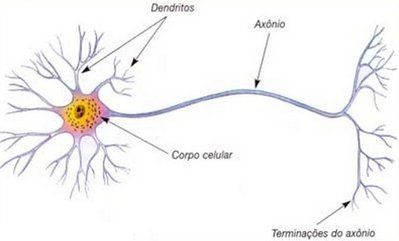
\includegraphics[width=0.5\linewidth]{images/neuronio-biologico.png}
    \caption{Estrutura de um neurônio: o sinal elétrico é levado do corpo celular para os terminais do axônio, onde é iniciada uma nova sinapse. Fonte: \cite{duarte2015interface}.}
    \label{fig:neuronio-biologico}
\end{figure}

Já o modelo matemático do neurônio artificial é uma simplificação dessa estrutura biológica. Ele é composto por várias entradas (dendritos) que recebem os valores x1, x2, x3, …, xn correspondentes as ativações dos neurônios anteriores, possui também um terminal de saída y que representa o axônio do neurônio biológico. Cada entrada do neurônio artificial possui um peso, chamado de peso sináptico, dado por w, os pesos servem para o neurônio artificial identificar o grau de relevância daquela entrada\cite{braga2014redes}. O neurônio artificial está representado na figura abaixo.

\begin{figure}[H]
    \centering
    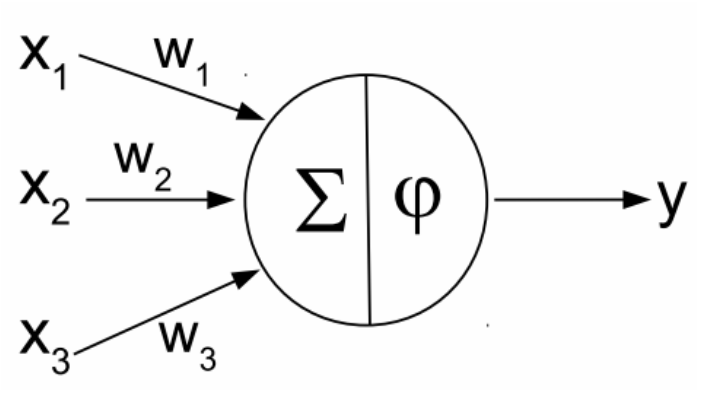
\includegraphics[width=0.5\linewidth]{images/neuronio-artificial.png}
    \caption{Representação esquemática de um neurônio artificial. As entradas \( x_1, x_2, x_3 \) são multiplicadas por seus respectivos pesos sinápticos \( w_1, w_2, w_3 \), resultando em uma soma ponderada. Essa soma é então processada por uma função de ativação, produzindo a saída \( y \). Fonte: \cite{giacomel2016metodo}}
    \label{fig:neuronio-artificial}
\end{figure}

\subsection{Função de ativação}

A função de ativação é responsável por gerar a saída do neurônio a partir da somatória das entradas com seus respectivos pesos. Esta função tem efeito apenas no neurônio em que ela está empregada.

As funções de ativação mais comumente utilizadas são: função logística e função tangente hiperbólica. A função logística ou sigmóide é dada por:

\[
\sigma(x) = \frac{1}{1 + e^x}
\]

Esta função de ativação foi amplamente utilizada em RNAs por ser mais parecido com a biologia pois como neurônios biológicos funcionam de forma binária, a função sigmóide é uma boa forma de modelar esse comportamento, já que assume valores apenas entre 0 e 1 \cite{facure2017funcoes}.

Similar a função sigmóide a função tangente hiperbólica varia de -1 a 1. \cite{facure2017funcoes} diz que por se aproximar mais da identidade a função tangente hiperbólica é melhor do que a sigmóide para as camadas ocultas. A função tangente hiperbólica é dada por:

\[
\tanh(x) = 2\sigma(2x) - 1 \quad \text{e} \quad \tanh'(x) = 1 - \tanh^2(x)
\]

\subsection{RNA Feedforward}

Também chamada de acíclica, neste tipo de rede todas as saídas dos neurônios estão direcionados para as entradas dos neurônios da próxima camada, a saída de um neurônio deve servir de entrada para todos os neurônios da camada superior e não é permitido o retorno da informação. Desta forma a rede segue em apenas um sentido, sempre para frente, como mostra a figura abaixo. Este tipo de rede é bastante utilizado em problemas não lineares para a classificação e reconhecimento de padrões \cite{ufsc2002introducao}.

Para que este estilo de RNA resolva um problema deve-se fornecer os dados para os neurônios de primeira camada, e desta forma os dados serão processados e enviados para as próximas camadas até chegar a camada de saída com o resultado obtido \cite{giacomel2016metodo}.

\begin{figure}[H]
    \centering
    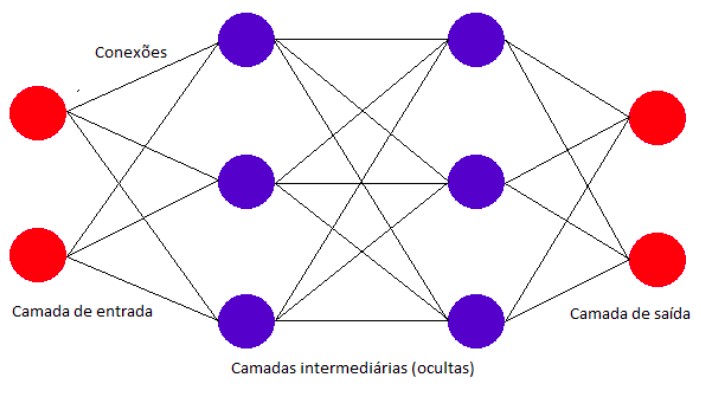
\includegraphics[width=0.5\linewidth]{images/rede-neural.png}
    \caption{Representação esquemática de uma rede neural artificial. Fonte: autor}
    \label{fig:rede-neural-artificial}
\end{figure}

\subsection{Fine-Tuning de Modelos de IA}

O fine-tuning, ou ajuste fino, é uma técnica essencial no campo da inteligência artificial, permitindo a adaptação de modelos pré-treinados a tarefas específicas com menor custo computacional e necessidade reduzida de dados rotulados. Essa abordagem é particularmente eficaz quando se busca especializar modelos de linguagem natural para domínios específicos, como o da saúde mental. Ao reutilizar o conhecimento adquirido durante o pré-treinamento em grandes corpora, o fine-tuning possibilita a personalização do modelo para contextos particulares, mantendo a eficiência e a eficácia do sistema \cite{ibm2023o}.

Entre as estratégias de fine-tuning, destaca-se o Domain-Adaptive Pretraining (DAPT), que consiste em reexplicar o modelo com dados não rotulados do domínio-alvo antes do ajuste supervisionado. Essa técnica melhora a compreensão do modelo sobre os padrões linguísticos específicos do novo domínio, resultando em melhor desempenho em tarefas subsequentes \cite{araujo2025fine}. Além disso, abordagens como o Parameter-Efficient Fine-Tuning (PEFT), incluindo métodos como LoRA (Low-Rank Adaptation), permitem ajustes eficientes ao modificar apenas uma pequena fração dos parâmetros do modelo, tornando o processo mais acessível em termos computacionais \cite{magalhaes2024entendendo}.

A escolha da estratégia de fine-tuning deve considerar fatores como o volume de dados disponíveis, a especificidade da tarefa e os recursos computacionais. Em contextos com dados limitados, como frequentemente ocorre na área da saúde, técnicas como o few-shot learning, que requerem poucas amostras para treinamento, podem ser particularmente úteis. Essas abordagens permitem que modelos pré-treinados sejam adaptados de forma eficaz a novas tarefas, mesmo com conjuntos de dados reduzidos, mantendo a precisão e a relevância das respostas geradas \cite{ibm2023o}.

Neste contexto de especialização da inteligência artificial para a área da saúde, acabamos enfrentando diversos desafios que vão além das questões técnicas, abrangendo aspectos éticos, legais e sociais. Um dos principais obstáculos é a escassez de dados de qualidade e devidamente rotulados, essencial para o treinamento eficaz dos modelos. A natureza sensível das informações de saúde, protegidas por legislações como a Lei Geral de Proteção de Dados (LGPD) no Brasil, dificulta o acesso a dados clínicos, limitando a capacidade de desenvolver modelos robustos e generalizáveis \cite{gee2024inteligencia}.

Além disso, a interpretabilidade dos modelos de IA é uma preocupação significativa na área da saúde. Profissionais e pacientes precisam compreender as decisões tomadas pelos sistemas para confiar em suas recomendações. No entanto, muitos modelos de aprendizado profundo operam como "caixas-pretas", dificultando a explicação de seus processos decisórios. Essa falta de transparência pode comprometer a adoção da IA em ambientes clínicos, onde a justificativa das decisões é crucial para a prática médica ética e responsável \cite{silva2023desafios}.

Outro desafio relevante é o potencial viés presente nos dados utilizados para treinar os modelos de IA. Dados históricos podem refletir desigualdades e preconceitos existentes no sistema de saúde, levando os modelos a perpetuar ou até amplificar essas distorções. Isso é particularmente preocupante em contextos de saúde mental, onde fatores socioeconômicos, culturais e étnicos influenciam significativamente os diagnósticos e tratamentos. Portanto, é fundamental implementar práticas de auditoria e validação contínua dos modelos, garantindo que suas decisões sejam justas e equitativas para todos os grupos populacionais \cite{souza2024desafios}.

\section{INTELIGÊNCIA ARTIFICIAL NA SAÚDE}

A Inteligência Artificial (IA) tem sido amplamente aplicada no setor da saúde, oferecendo soluções que vão desde a análise preditiva até o suporte à tomada de decisões clínicas, passando pela automação de relatórios e extração de informações relevantes a partir de grandes volumes de dados clínicos. A capacidade da IA em lidar com dados não estruturados, como textos de prontuários, laudos médicos e anotações de sessões terapêuticas, possibilita uma transformação significativa na forma como os profissionais de saúde realizam seu trabalho \cite{brasil2022inteligencia}.

Entre as principais aplicações da IA na saúde está a geração automatizada de relatórios clínicos e terapêuticos. Por meio do uso de modelos de linguagem natural, como os processadores de linguagem natural (NLP), é possível resumir e estruturar informações de prontuários eletrônicos, facilitando a elaboração de diagnósticos, laudos e documentos legais. Essa abordagem não apenas economiza tempo dos profissionais, mas também reduz erros e padroniza a documentação clínica \cite{silva2021aplicacao}.

Outro campo de aplicação relevante é a extração de informações de documentos e registros clínicos. Ferramentas de IA podem ser treinadas para identificar sintomas, diagnósticos prévios, medicamentos prescritos e outras informações sensíveis, mesmo em textos longos e não padronizados. Segundo o Ministério da Saúde (2021), esse tipo de tecnologia tem grande potencial para apoiar o monitoramento epidemiológico, auditorias clínicas e a continuidade do cuidado ao paciente.

Além disso, sistemas inteligentes também têm sido empregados como assistentes digitais para apoiar médicos, psicólogos e demais profissionais da saúde no processo de tomada de decisão clínica. Tais sistemas são capazes de sugerir tratamentos com base em diretrizes clínicas, histórico do paciente e dados extraídos automaticamente de registros anteriores, oferecendo suporte baseado em evidências científicas \cite{conass2020inteligencia}.

\section{MODELO DE IA QUE SERÁ UTILIZADO}

 plataforma proposta neste trabalho utilizará um modelo de linguagem baseado em redes neurais do tipo transformer, voltado para aplicações de Processamento de Linguagem Natural (Natural Language Processing – NLP), com o objetivo de automatizar tarefas como a elaboração de relatórios terapêuticos, extração de informações de textos clínicos e assistência ao profissional da saúde mental. O modelo selecionado para essa finalidade é o LLaMA (Large Language Model Meta AI), desenvolvido pela Meta AI Research.
 
O LLaMA é uma família de modelos de linguagem autoregressivos que seguem a arquitetura transformer, proposta por Vaswani et al. (2017), e que se destaca por sua capacidade de capturar longos contextos e gerar texto de forma coerente e contextualizada. Os modelos LLaMA foram projetados com foco em eficiência, permitindo que pesquisadores e desenvolvedores utilizem modelos de linguagem de última geração sem depender exclusivamente de grandes infraestruturas computacionais ou serviços de nuvem \cite{touroude2023llama}.

Para o presente trabalho, será utilizada a versão LLaMA 2, com enfoque no modelo Zephyr-7B-alpha, que conta com aproximadamente 7 bilhões de parâmetros e foi treinado com técnicas de instrução supervisionada (instruction tuning), o que o torna adequado para responder a perguntas, gerar textos formais e executar tarefas orientadas por comandos. Este modelo será empregado em versão quantizada (por exemplo, Q5_K_M), utilizando a biblioteca llama.cpp, que permite sua execução em dispositivos locais, mesmo com recursos computacionais limitados, como notebooks com menos de 16 GB de RAM.

A quantização consiste em uma técnica de compressão do modelo que reduz o uso de memória e acelera a inferência, com perda mínima de precisão, sendo especialmente útil em ambientes edge computing ou quando se busca maior controle sobre os dados sensíveis, como ocorre no contexto clínico (DE VINCENTIS et al., 2023). A execução local do modelo quantizado viabiliza o cumprimento das exigências da Lei Geral de Proteção de Dados (LGPD), garantindo que nenhum dado clínico seja transmitido para servidores externos ou terceiros \cite{brasil2018lei}.

Além disso, o modelo será adaptado ao domínio da saúde mental por meio de um processo de prompt tuning com dados sintéticos representativos da prática clínica, incluindo exemplos de anotações de sessões, encaminhamentos e relatórios psicológicos. Isso permitirá ao modelo aprender padrões e estruturas linguísticas específicas da psicologia clínica, aumentando sua eficácia como ferramenta de apoio profissional.

A escolha do LLaMA se justifica por sua robustez, facilidade de customização, compatibilidade com ambientes de alta confidencialidade e por ser de código aberto. Sua utilização permite a construção de uma solução de NLP eficaz, ética e segura, com potencial de auxiliar psicólogos e psiquiatras em tarefas cotidianas, otimizando tempo e padronizando a produção de documentos clínicos.

\section{NORMATIVAS E LEGISLAÇÃO SOBRE DADOS MÉDICOS}

A manipulação de dados médicos no Brasil é regulada principalmente pela Lei nº 13.709, de 14 de agosto de 2018 — a Lei Geral de Proteção de Dados Pessoais (LGPD), que classifica informações sobre saúde como dados sensíveis. Essa categoria exige tratamento especial, garantindo maior proteção contra acessos indevidos, vazamentos ou uso indevido das informações \cite{brasil2018lei}.

A LGPD determina que o tratamento desses dados só pode ser realizado mediante consentimento explícito do paciente ou quando indispensável para prestação de serviços de saúde, desde que conduzido por profissionais ou instituições autorizadas (art. 11, I e II). Isso se aplica diretamente à plataforma proposta, que deverá operar em conformidade com essas diretrizes para garantir a legalidade do armazenamento e do processamento de documentos clínicos.

Além do consentimento, a lei impõe princípios como segurança, necessidade, transparência e prevenção, exigindo que sejam adotadas medidas técnicas e administrativas para proteger os dados (art. 6º e art. 46). Entre essas medidas, destacam-se o uso de criptografia, autenticação de usuários e controle rigoroso de acesso.

O respeito às normativas da LGPD não apenas evita sanções legais, como também reforça a confiança dos profissionais de saúde e pacientes no uso da tecnologia. Assim, o cumprimento das exigências legais deve ser considerado um dos pilares fundamentais do desenvolvimento da plataforma.

\section{MODELOS DE SISTEMAS PARA ARMAZENAMENTO DE DADOS NA SAÚDE}

Atualmente, diversos sistemas são utilizados para o armazenamento e gerenciamento de dados na área da saúde, incluindo os Prontuários Eletrônicos do Paciente (PEP), Sistemas de Informação Hospitalar (SIH) e plataformas de gestão clínica. Esses sistemas têm como objetivo organizar informações médicas, facilitar o acesso por profissionais autorizados e garantir a continuidade do cuidado ao paciente. No entanto, muitos deles ainda enfrentam desafios significativos relacionados à interoperabilidade, segurança e usabilidade.

Um dos principais obstáculos observados nesses modelos é a fragmentação dos dados. Com frequência, informações sobre um mesmo paciente ficam dispersas entre diferentes instituições ou sistemas, dificultando o acesso completo ao histórico clínico. Além disso, muitos sistemas legados carecem de integração com tecnologias modernas, como Inteligência Artificial (IA) e APIs de assinatura digital, o que limita seu potencial de automação e análise de dados.

A segurança também é uma preocupação central. Sistemas que não adotam criptografia de ponta a ponta, autenticação robusta ou controle de acesso baseado em perfis estão mais suscetíveis a violações de privacidade. Isso é especialmente problemático em um contexto de crescente digitalização e em conformidade com a Lei Geral de Proteção de Dados (LGPD), que exige medidas rigorosas para a proteção de informações sensíveis \cite{brasil2018lei}.

Nesse cenário, há espaço para o desenvolvimento de soluções mais modernas e seguras, com foco em modularidade, armazenamento criptografado, integração com ferramentas de NLP e possibilidade de execução local dos serviços.

\section{TRABALHOS RELACIONADOS}

Diversos estudos brasileiros têm se dedicado ao desenvolvimento e aprimoramento de plataformas digitais voltadas à saúde, com foco na utilização de técnicas de Inteligência Artificial (IA), principalmente o Processamento de Linguagem Natural (NLP), para a extração e estruturação de dados clínicos. \citeonline{souza2024recuperacao}, por exemplo, exploraram o uso de PLN para recuperar informações relevantes de prontuários ginecológicos, destacando o potencial de reutilização de anotações clínicas não estruturadas com o objetivo de alimentar repositórios de dados e apoiar pesquisas e gestão em saúde. De forma semelhante, \citeonline{santos2024classificacao} aplicaram modelos baseados em BERT para a previsão automática de códigos CID a partir de relatórios de internações neonatais, demonstrando a aplicabilidade de IA na automatização de classificações diagnósticas.

No entanto, ambos os estudos têm como foco principal a aplicação de NLP em domínios específicos da saúde (ginecologia e neonatologia) e em contextos hospitalares mais amplos, sem considerar o armazenamento seguro e individualizado de documentos terapêuticos voltados à saúde mental, especialmente em psicologia clínica. 

No que se refere à segurança da informação, \citeonline{magnagnagno2020seguranca} analisaram práticas adotadas em ambientes hospitalares brasileiros, observando a utilização de criptografia em comunicações e o uso de certificados digitais da ICP-Brasil para assinatura de prontuários eletrônicos. \citeonline{tertulino2024privacidade} também destacaram a importância da autenticação forte, da rastreabilidade dos acessos e da conformidade com a LGPD como aspectos essenciais na construção de sistemas seguros. No entanto, tais trabalhos se concentram em sistemas hospitalares amplos, sem considerar soluções mais enxutas e especializadas que atendam diretamente profissionais autônomos ou clínicas de psicologia.



% 
%--------- FIM FUNDAMENTAÇÃO------------
%